\documentclass[11pt]{article}

\usepackage{fullpage}
\usepackage{graphicx}

\begin{document}

\title{\vspace{-1.5\baselineskip}ARM11 Final Report}

\author{Aahil MEHTA, Miroslav LAMBREV, Radostin PETROV, Ruari PHIPPS}

\maketitle

\section{ARM11 emulator and assembler}
\begin{minipage}{0.6\linewidth}
\subsection{Emulator implementation}

For initial implementation of the emulator, check \texttt{doc/Checkpoint.pdf}. We have since modified the emulator by introducing a \texttt{decode.c} module, that depends on a \texttt{decode.h} header, which serves to process and decode the different types of instructions. That way we have split the work done by \texttt{execute.c} roughly in half and spread it between it and \texttt{decode.c}. The dependency graph for the emulator has since slightly changed.

\subsection{Assembler implementation}

Our assembler has the following structure:
\begin{itemize}
    \item The \texttt{assemble.c} file contains the \texttt{main} function, which takes the incoming assembly file and the output binary filename as arguments. It then reads data from the file line by line, generating a symbol table in the first pass of the code. In the second pass we generate the binary encoding for each instruction and then write it into memory. The type of instruction is decoded by tokenizing the strings mnemonic and passing it to a look-up table called the parse type table which returns an index to an array of function pointers that will be used to parse the instruction. After that has been successfully done, we save the memory into a binary file.
    \end{itemize}
    \end{minipage}
\hspace{0.05\linewidth}
\begin{minipage}{0.35\linewidth}

\centering

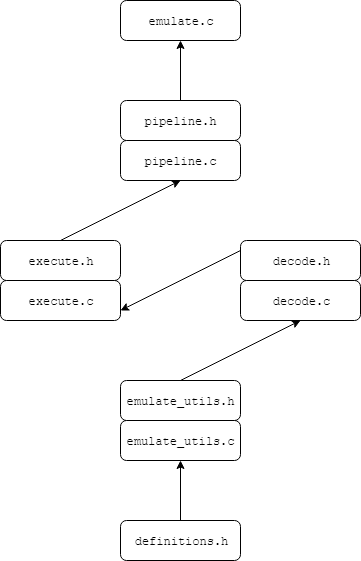
\includegraphics[scale=0.8]{diagrams/EmulatorDependencies.png}
\caption{Figure 1: Dependency Diagram for \texttt{emulate.c}}

\end{minipage}
    \begin{itemize}
    \item The \texttt{parser.c} file has all the parsing functions for all types of instructions (special included), as well as functions to parse the register and the expressions (in the case of immediate values).
    \end{itemize}
\begin{minipage}{0.6\linewidth}
    \begin{itemize}
    \item \texttt{assembler\_utils.c} contains helper functions that we use in the assembler to prevent duplication of code or inline complexity, such as functions to generate a move instruction, to generate the offset in branch instructions, writing 4 bytes to memory and saving the memory into the output file.
    \item The \texttt{symbol\_table.c} file has all functions connected to our \texttt{Symbol\_Table} ADT, defined in \texttt{symbol\_table.h}. The structure represents a single linked list of \texttt{(String, Integer)} pairs. Functions on the table include ones for initializing the table, adding entries to it, obtaining the \texttt{Integer} value associated with a \texttt{String} key, and creating new tables as well as storing arbitrary data in them.
\end{itemize}
\par For all of the \texttt{.c} files in our implementation (except \texttt{assemble.c}) we have their respective header file, containing the dependent libraries. We also use the header \texttt{definitions.h} like in \texttt{emulate.c}, where we have defined all the constants and type definitions we have used in our assembler.
\end{minipage}
\hspace{0.05\linewidth}
\begin{minipage}{0.35\linewidth}

\centering
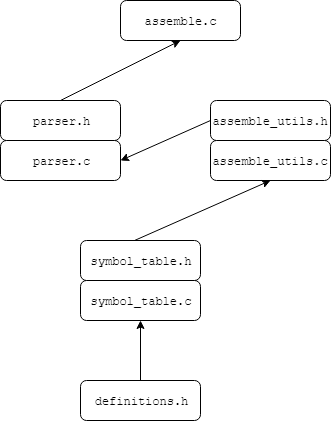
\includegraphics[scale=0.8]{diagrams/AssemblerDependencies.png}
\caption{Figure 2: Dependency Diagram for \texttt{assemble.c}}

\end{minipage}

\subsection{General purpose IO on a Raspberry Pi}
We initially extended \texttt{emulate.c} to support the gpio functions and after we passed the tests on the test suite, we tested it successfully on the Raspberry Pi. \texttt{/programs/gpio.s} contains the assembly code we used for this part. We later created a \texttt{gpio.c} in packaged with the extension in directory \texttt{/extension/src/gpio.c} which supports setting and clearing all available gpio pins as well as a delay function.

\subsection{Code Styling and Testing}
\paragraph{Style Guide} We have thoroughly discussed code styling with our mentor and amongst ourselves and we have decided to use the \textbf{Clang-Format Style}, which comes as a default in the CLion IDE. We made sure we commented our code frequently and efficiently to ensure maximum readability between group members.
\paragraph{Testing} We created our own unit tests in a source file located in \texttt{/src/tests.c}, which was used to debug parts of our assembler locally. The program uses standard output to test that our helper functions are working accordingly. The file was also used to test functions such as \texttt{strtok\_r} which had a relatively complicated documentation. This type of debugging proved useful when testing for memory leaks as well, however, for that we mainly relied on \texttt{valgrind} for checking errors.


\section{C120.3 Extension: Bare Metal Roguelike on a Raspberry Pi}
\subsection{Introduction}

The extension we chose to create is a Roguelike Bare Metal game that runs on the Raspberry Pi. There were two parts to our project: we first created the framework, which allowed us to create games and output them on a monitor. Using it we could create any game. The second part was creating a Roguelike game to demonstrate the potential of Procedural Generation and the power of GPU of the Raspberry Pi.


\subsection{Implementation}
\subsubsection{Creating a Game Engine Framework}
Our framework has the following file structure:
\begin{itemize}
    \item \texttt{start.s} sets the stack pointer, enables the L1 cache and calls \texttt{\_cstart()} in \texttt{cstart.c}
    \item \texttt{cstart.c} is used to zero out the BSS and call \texttt{main} from \texttt{run.c}. This is done to set uninitialized global variables (which are stored in the BSS) are zero.
    \item \texttt{run.c} consists of the main function which contains the game loop, ie. \texttt{start()}, \texttt{update()}, \texttt{draw()} functions.
    \item \texttt{graphics.c} is a graphics library we created to draw different types of shapes and text on the screen by modifying the framebuffer. Functions allow the user to draw pixels, lines, rectangles, characters and strings to the screen.
    \item \texttt{fb.c} contains methods to initialize the frame buffer and clear it, as well as helper functions to retrieve its size and depth.
    \item \texttt{mailbox.c}, has functions to write messages via a channel to the mailbox (which sends data to the GPU), and read messages from it. This is done in accordance to the Raspberry Pi documentation.
    \item \texttt{timer.c} contains a frame counter and a sleep method to delay the code.
    \item \texttt{random.c} consists of a random number generator
    \item \texttt{resources.c} is a store of resources such as fonts and images which are stored as arrays of integers
\end{itemize}

For all the \texttt{.c} files, except \texttt{cstart.c}, \texttt{run.c} and \texttt{gpio.c} we have a respective header file, which contains function declarations, as well as definitions for the various structures that we have used.

\subsubsection{Roguelike game creation}
Although this part is unfinished, our progress on the game is the following:
\begin{itemize}
    \item \texttt{map\_generator.c} consists of a function \texttt{generate\_map} and several helper functions. This procedurally generates a 2D Roguelike map and stores it in a 2D array, where 1 represents a wall tile and 0 represents a floor tile.
\end{itemize}

\subsubsection{Testing}
Testing our work proved to be challenging due to not being able to use some essential C libraries, as well as being unable to output to the console. Initially, we debugged our program by using the GPIO output to see how far the execution of the program got (i.e. one blink equals one step). 
\par However, since we were creating a graphics library, the code functionality was dependent on the monitor output. Hence we could simply debug our program, by analyzing an arbitrary output, which utilized all the functions. Being able to draw strings later on significantly helped us debug.

\subsubsection{Future Work}
For future work in our extension we aim to use our framework to create a Bare Metal Roguelike implementing the map generator we have already created. We will implement turn based player motion using an input from either a joystick or a keyboard. We plan to create an enemy generating script and, if left with enough time, use images and implement animations.


\section{Project Evaluation}

\subsection{Group Workflow and Organization Reflections}

Our group organization started with planning out the project structure and interpreting the information from the spec. We used a shared Google Document to make knowledge transfer accessible and have a place to refer to if we had any questions regarding the spec. We created a Discord server for communication with channels for the different parts of the project. This helped focus on each part individually and reflect on our progress.
\par After deciding on the data types, variables and our general structure, we started pushing our work to git. We split the work into smaller chunks and assigned tasks to team members. We used both git and the Google Document to raise issues and plan ahead. Although we assigned different jobs to group members, we would often collaborate or switch roles, if the person was having difficulties with their part of the work.
\par We initially had problem with our teamwork and it took some time for each member to fully integrate into the team. However, after a couple of team meetings our workflow greatly improved and we started making use of git more efficiently. Our team has a good mix of skills that were all necessary for the execution of this project. Some members were more experienced on the implementation side of the project, having more programming experience, while others had an understanding of the technical side, consisting of testing, compiling, etc. Our skills complemented each other and whenever someone encountered a problem, there was always some member from the team that could help with it.

\paragraph{Advantages in our workflow} Explaining and reinterpreting the spec, so that each member can understand the core of our project, was very beneficial for the team. Having a place to refer to when you have a question and immediately receive an answer was very convenient for us to get work done efficiently. We also set ourselves deadlines for the milestones throughout the project. This helped the team stay on track and keep the organization intact .

\paragraph{Disadvantages in our workflow} Not being familiar with git, it was a significant challenge to figure out how we can all work on the same code remotely. Before our first commit, we had already done a good amount of work, but we had to all store the same file in the cloud, so that we can work on it. For next time we should make sure to use git a lot more efficiently, make more sensible branches and document the code. We would also delegate tasks more strictly, so that no one on the team is without a task and is confused with what they should or could be doing at any given time.

\subsection{Individual Project Reflection}

\paragraph{Aahil MEHTA} I started out this project with no experience in C and not knowing some of my teammates, however, over the course of the past few weeks our team has formed a strong bond and progressed far beyond we imagined we would in the given time. I feel I have been a valuable member of the team, bringing my experience with bit-shifts, planning, and eagerness to learn to the mix. As leader, I made sure we had a thorough plan for each part of the project before we started programming, and I tried to split it into tasks which we could complete one by one. 
\par One of my shortcomings was jumping on tasks myself before understanding them completely, which led to inefficient code in many places. If I had to do it over, I would be more specific in defining tasks, I would be more careful with my choice of data types, and I would use debuggers such as \texttt{valgrind} more often.
\par In the last 3 weeks, I have learnt far more C than I ever expected learning this term, my proficiency with git has improved a lot, I have gained a valuable set of skills in debugging, I have been able to study a fair amount of arm architecture, and I have had the chance to program a bare-metal game. There is no doubt it has been an amazing experience, and I have enjoyed every moment.

\paragraph{Miroslav LAMBREV} I am very satisfied with the overall performance of our group. I believe that we successfully managed to utilize the strengths of every team member which allowed us to work on areas we are confident in and learn from the others on areas we are not as experienced in.
\par One of my weaknesses going into the project as a JMC student was my lack of prior knowledge of Computer Architecture. During the first few days after the specification was released, I found it very challenging to understand most of the concepts that were introduced. However, my teammates gave thorough answers to my questions and I slowly started building confidence and began tackling the emulator.
\par This leads me to one of my strengths. As long as I have a clear idea of what my program is supposed to do, I believe that I am very good at coming up with a working solution (not always the most practical one). That skill allowed me to provide my team with a solid starting point for the implementation of the emulator on which we would build on and improve.
\par Another trait of mine is my pedantry. I am rarely fully satisfied with the written code and always look for improvements whether it is the implementation or the readability which led to my responsibility of polishing the code after it was complete.
\par The next time I work on a group project I wish that I would be more confident in my computing knowledge and actively take part in the discussions regarding the implementation of the more complicated parts of the project.

\paragraph{Radostin PETROV} Looking back on our work, I feel very happy with the progress we have made. In the beginning, there were group members who did not even know each other, however, by the end we had created this small scale project with potential to be extended in any way imaginable.
\par Although, the programming experience between group members varied largely, there was absolutely no conflict between group members and we were able to keep our work very professional. I strongly insisted on professionalism to some extent. I made sure to take initiative in creating the communication channels, as I suspected communication would be a challenge. Although myself unfamiliar with git, I pushed the team to use and learn it, as I believed the tools from the platform would prove very beneficial to our work down the road.
\par I was strongly in favor of planning, pushing my team to plan ahead of time and I made sure that each team member was aware of the tasks and the deadlines. We set ambitious internal deadlines, so that we could keep the motivation for work in the team. I believe this type of organization to be one of my strongest sides.
\par A weakness of mine was likely the lack of knowledge of the C programming language. I was timid in using the language in the start of the project. I did not write as much code as other team members for that matter, but I made sure that I knew and understood the code that they have written. I am happy to say that through observing their code I have learnt a lot about programming practices in general.
\par I believed my role in the team to be very significant and I would continue this practice in future team projects. What I would change is that I will try to contribute a lot more in the programming part of the project, because I believe that I have gained enough experience and knowledge from this project.

\paragraph{Ruari PHIPPS} I think I managed to fit into the group very well. I did not know the members of the group much beforehand, but I felt comfortable to get across my ideas, engage in discussion and to learn from the other team members as the group had a very friendly feeling.
\par In terms of my strengths, I had a small prior knowledge of git before the project, I did not think this would be a strength, but I was able to use git in a clear way and was able to help others to do so properly, this really helped our group structure and organise our code. I believe another one of my strengths was being able to organise the code into sections, and comment what was expected in each part, this was very useful as it made it easier for people to work on the project.
\par One of my weaknesses going into the project was my knowledge of C. I had to get help from other people in the group and relied on them to tackle some of the more complex parts of the project, but my understanding of C did improve a lot throughout the project and feel I still managed to contribute a decent amount to the project.
\par The next time I am in a group project, I will maintain the way I organised the code to keep a good code structure that allows people to easily add and work on different parts of the code separately. However, next time I would change the way I work on the code and challenge myself to work on some of the more difficult parts as well as taking some leadership and directing how things should be done.


\end{document}
